\documentclass{article}
\usepackage[utf8]{inputenc}
\usepackage[T1]{fontenc}
\usepackage{hyperref}
\usepackage{url}
\usepackage{booktabs}
\usepackage{amsfonts}
\usepackage{nicefrac}
\usepackage{microtype}
\usepackage{graphicx}
\usepackage{xcolor}
\usepackage{subcaption}
\usepackage{lipsum}
\usepackage[a4paper, total={6in, 8in}]{geometry}
\usepackage{biblatex}
\documentclass{article}
\graphicspath{ {./images/} }
\usepackage{float}


\title{Public Safety Power Shut-off GRIP Module Documentation}
\setlength{\parindent}{0pt}
\setlength{\parskip}{0.7em}

\begin{document}

\maketitle

\section{Motivation}

Public safety power shut-off (PSPS) events to prevent wildfires are becoming increasingly frequent as climate change exacerbates and extends the fire season and as development continues to expand into areas where fires are a natural feature of the ecosystem. This combination of increased fire probability, many people's lives and livelihood at risk, and more assets facing potential destruction contributes to a large risk of wildfires. Recent major events caused by electric distribution lines have made it clear to utilities that this risk is a growing liability. While the costs of fire damage can be high, the costs associated with cutting off power to customers are significant. This PSPS optimization problem is an important one to solve because it is a key problem utilities and public safety officials face today when deciding how to balance the risk of catastrophic fires with the obligation to serve electricity demand. 

Our work builds off of the work in Rhodes et al.$[1]$ to implement a Mixed Integer Linear Program (MILP) that minimizes wildfire risk and lost customer load hours in a distribution system when scheduling a PSPS event. The optimization algorithm takes into consideration the wind conditions, vegetation fire risk, customer locations, and historical fire risk data when determining the optimal node(s) to switch power off. Our problem is tested on an IEEE 123 bus system placed in a high fire risk zone, as well a PG&E distribution system in Napa, CA.

Because the acceptance of wildfire risk is a subjective parameter, we use the weighted sums method of multi-objective optimization to explore the pareto-frontier of the optimal PSPS event. This will allow us to compare how PSPS events change when accounting for a range of risk tolerance.

\section{Methods}
\subsection{Objective function}

Our model is a bi-objective temporal network model in which customer electricity service is co-optimized with fire risk reduction. A description of the model's objective function can be found below. The decision variables in our model, $x_{t,a}$, are binary variables representing the switch status of each sectionalized area $a$ at time $t$.

\begin{equation}
    \min_{x} {\sum_{t}^{T}\sum_{a}^{A} [x_{t,a} * R_{t,a} * (1 - \alpha) - x_{t,a} * C_{t,a} * \alpha}]
\end{equation}

where:
\begin{itemize}
    \item $x_{t,a}$ : Switch status of area $a$ at time $t$
    \item $R_{t,a}$ :  Fire Risk of area $a$ at time $t$
    \item $\alpha$ : Hyperparameter representing the acceptance of wildfire risk
    \item $C_{t,a}$ : Customers of area $a$ at time $t$ $[Customer-hrs]$
    \item $A$ : Set of all grid sectionalized areas
    \item $T$ : Set of all timesteps
\end{itemize}

\subsection{Constraints}
Our objective function is constrained so that the status (0 or 1) of each switch $x_{a}$ in set $A$ depends on the positions of all switches upstream of it in the distribution system. This constraint ensures that a section of the grid cannot be \emph{islanded} or turned on without being connected to a path to the substation.

\begin{equation}
     x_{a} \leq {\sum_{d}^{D} x_{d}}  \;\;\;\;  \forall \; a \in A \;\; and \;\; a \not\in  S
\end{equation}

where:
\begin{itemize}
    \item $x_{a}$ : Switch of area $a$ in set $A$
    \item $x_{d}$ : Switch of area $d$ that area $a$ is connected to
    \item $D$ : Set of all switch areas that area $a$ is connected to
    \item $S$ : Set of all source (substation) switch areas $a$ \in $A$

\end{itemize}

\section{Data Preparation}

\subsection{Fire Risk}

Fire risk is defined as the product of the area level USGS Fire Potential Index and Ignition Probability. The USGS fire potential index and the ignition potential will be combined to represent the fire risk in each area $a$ at time $t$. The total fire risk will be represented by $R_{t,a}$ for each length of powerline and then aggregated to each switch level area.

\begin{equation}
    R_{t,a} = FPI_{t,a} * IGP_{t,a}
\end{equation}where:
\begin{itemize}
    \item $FPI_{t,a}$ : Normalized sum of USGS Fire Potential index of area $a$ at time $t$
    \begin{equation}
        FPI_{t,a}  =  \frac{\sum_{n}^{N_a}FPI_{t,n}}{\max(FPI_A)}
    \end{equation}
    \item $IGP_{t,a}$ : Normalized sum of Ignition Potential of area $a$ at time $t$
    \begin{equation}
        IGP_{t,a}  =  \frac{\sum_{n}^{N_a}IGP_{t,n}}{\max(IGP_A)}
    \end{equation}

\end{itemize}
The  Fire Potential Index $FPI$ is an index produced by the US Geological Service which describes vegetation flammability on a scale 0-248 at 30 meter resolution. The FPI inputs include: maximum live/dead fuel ratio, dead fuel extinction moisture, fuel model, wind reduction factors, Normalized Difference  Vegetation Index (NVDI), Relative Greenness, 10-Hour Dead Fuel Moisture, Wind Speed, Rain, Dry Bulb Temperature. Each node's geographic point in the simulation is assigned a FPI according to the daily USGS FPI value. This daily value is re-sampled to an hourly level with a quadratic interpolation between days. Each node is then aggregated and normalized to the area or \emph{group\_id} which represents a section of the grid.

The USGS Fire Danger Forecast also include products for Large Fire Probability and Fire Spread Probability. These data streams are currently not used in this implementation of PSPS optimization, but should be included in future iterations. 

\begin{figure}[H]
    \centering
    \begin{minipage}{0.35\textwidth}
        \centering
        \includegraphics[width=1\textwidth]{FPI_USGS.png}
        \caption{USGS Fire Potential Index Map of Southwest US.}
    \end{minipage}
\end{figure}

The USGS FPI provides information as to how likely a spark will build into a fire given the above listed conditions, in order to gauge the likelihood of a spark from distribution system power lines we built a logistic regression model of ignition probability. This logit model was trained PG&E's fire ignition data from 2014 to 2021 $[2]$, and historical wind and weather data in PG&E service territories from the Meteostat Python package $[3]$. In this 7 year window there were 2480 ignition events reported to be caused by vegetation contact with power lines.  

Because we only had data on presence of fire ignition events, and the logistic model necessitates absence data, we constructed a pseudo-absence data-set from randomly sampled wind values in the month prior to each ignition event at each event location. We utilized the Meteostat weather API to pull the historical weather data at each PG&E ignition point.  The Logit model scored an Area Under Curve (AUC) score of 0.64 as seen in the Receiver Operator Curve (ROC) below. This AUC is marginally better than a random guess (AUC = 0.5). The simple model only uses wind-speed to predict ignition, and future models should include vegetation height, vegetation cover density, pole height, line voltage.


\begin{equation}
    Pr(Ignition=1| X_{wind}) = {\frac{exp(\beta_0 + \beta_1X_{wind})}{1 + exp (\beta_0 + \beta_1X_{wind} )}}
\end{equation}


\begin{figure}[H]
    \centering
    \begin{minipage}{0.55\textwidth}
        \centering
        \includegraphics[width=1\textwidth]{ROC Curve.png}
        \caption{ROC Curves of Logit models.}
    \end{minipage}
\end{figure}

\subsection{Options}

\subsubsection{GLM -> JSON Option}

The JSON file option takes the output of GLM -> Json conversion from gridlab-d. The Json file is read in the $loadJsonData()$ function to convert the Json file to a pandas dataframe to be populated with fire potential index and weather data.  

% \begin{table}[]
%     \centering
%     \begin{tabular}{c c}
%          node & Name of system object\\
%          class & defines type of object (substation, overhead_line, meter, load)\\
%          group id & defines ID of sectionalizable area \\
%          from/to & \\
%          load & \\
%          lat & \\
%          long & \\
%          length & \\
%          height
%     \end{tabular}
%     \caption{Caption}
%     \label{tab:my_label}
% \end{table}


The Json option has been pre-loaded with an example IEEE123 bus test system. This IEEE123 bus system has five sectionalized areas and is placed in the central valley near Bakersfield, CA. 

The PSPS module has not been tested with other JSON files and is likely to encounter some compatability issues when tested with JSON files that have slight differences compared to the IEEE123 example file.

\subsubsection{CSV Option}
 The PSPS module can also be run with a CSV file that includes the information for fields: group-id, lat, long, customerCount, and class. The current implementation assumes all the points in the CSV file are overhead lines and assign the class value to overhead lines. This choice is made since the CSV file upload is take from the PG&E Integrated Capacity Analysis map described in the Distribution System Topology section below. The only objects that are assigned in the psps workflow fire risk are overhead lines. 
 
 \subsubsection{Historical and Forecast Weather Data Options}
 There are options to analyze historical and forecasted fire risk. The difference in the two options is in the source of wind data. Forecasted fire risk takes wind from the gridlab-D $noaa_forecast$ tool while the historical fire risk option uses the gridlab-D $meteostat_weather$ tool. As currently implemented the historical weather data analysis is \bold{much} faster than the NOAA forecast tool. This is due to the implementation of the $meteostat_weather$ package which caches the data previously accessed as well as the psps package which generates a sequence of weather station ID's for which to map weather data to. The NOAA forecast function must call the tool for each of the potentially thousands of data points. 

\subsection{Distribution System Topology}

There are two options for uploading the distribution system for PSPS analysis. First, loading a JSON file created from Gridlab-D GLM file. Second, the CSV option with pre-sampled points along the distribution system. 


PG&E provides electricity to about 72,000 customers in Napa County. To construct topology for the area, we created a simplified version of PG&E’s distribution system using QGIS $[9]$. The main layer is a modified version of PG&E’s Integration Capacity Analysis (ICA) shapefiles $[5]$, parsed down to include the 2,746 kilometers of lines organized into 31 distribution feeders drawing power from the 8 substations within Napa County. Lines extending from these substations beyond the county line were included, and lines from substations outside of Napa County were excluded. Additionally, feeders were assumed to be independent from one another. Due to the complexity and data availability associated with power flow modeling, potential connections between feeders (beyond the substation) were ignored. As distribution lines are the primary source of wildfire risk, transmission lines bringing power to the substations were not integrated into the model. The result of this simplification is a set of 31 independent feeders with power flowing one way from substation to end nodes.

These feeders were divided into 102 subfeeders using 84 current and planned sectionalizing devices within our topology. The approximate\footnote{Data were not available for download, only through PG&E's interactive map online. Devices were represented as points that disappear when zooming in. Fortunately, in most cases, ICA shapefiles have rectangular loops at the likely device locations, making digitizing these points relatively simple and reliable.} locations of these devices were collected from PG&E’s PSPS online map interface $[6]$ and manually digitized onto the modified ICA map.

With these measures in place, PG&E's ability to minimize the number of customers with shutoffs greatly increases. Without such devices, when fire risk reaches a certain threshold, PG&E would have to shut off the entire feeder - only part of which is experiencing dangerous conditions. By segmenting the feeders, PG&E would be able to restrict the shutoffs to an outer section on a windy ridge without also shutting down customers in a low-risk area upstream, for example. To allocate the feeder-level customer counts from the ICA data, subfeeder customer counts were geospatially weighted by population $[8]$ within 500 meters of the line vectors. The resulting topology was sampled into about 92,000 points at 30-meter increments, which are used as the input values for the optimization model.

Although the ICA shapefiles are an incredibly valuable resource, due to security concerns and a primary purpose of informing interconnection of distributed energy resources, some data is either redacted or missing. In order to integrate these files into the model, the following changes were made to the data:

\begin{enumerate}
\item Applied an 8-meter buffer to the distribution line vectors to connect and group disconnected line segments
\item Cleaned missed and additional connection issues created by the buffering process - without a properly connected network, the algorithm used to segment the feeders does not work
\item Divided the cleaned buffer network feeders into subfeeder segments using orthogonal line intersections at the sectionalizing device locations
\item Repaired features and layer errors as needed
\item With the completed buffer subfeeder network layer, split the original line vectors into subfeeders
\item Edited connections and validated final subfeeder line layer
\end{enumerate}

\begin{figure}[H]
    \centering
    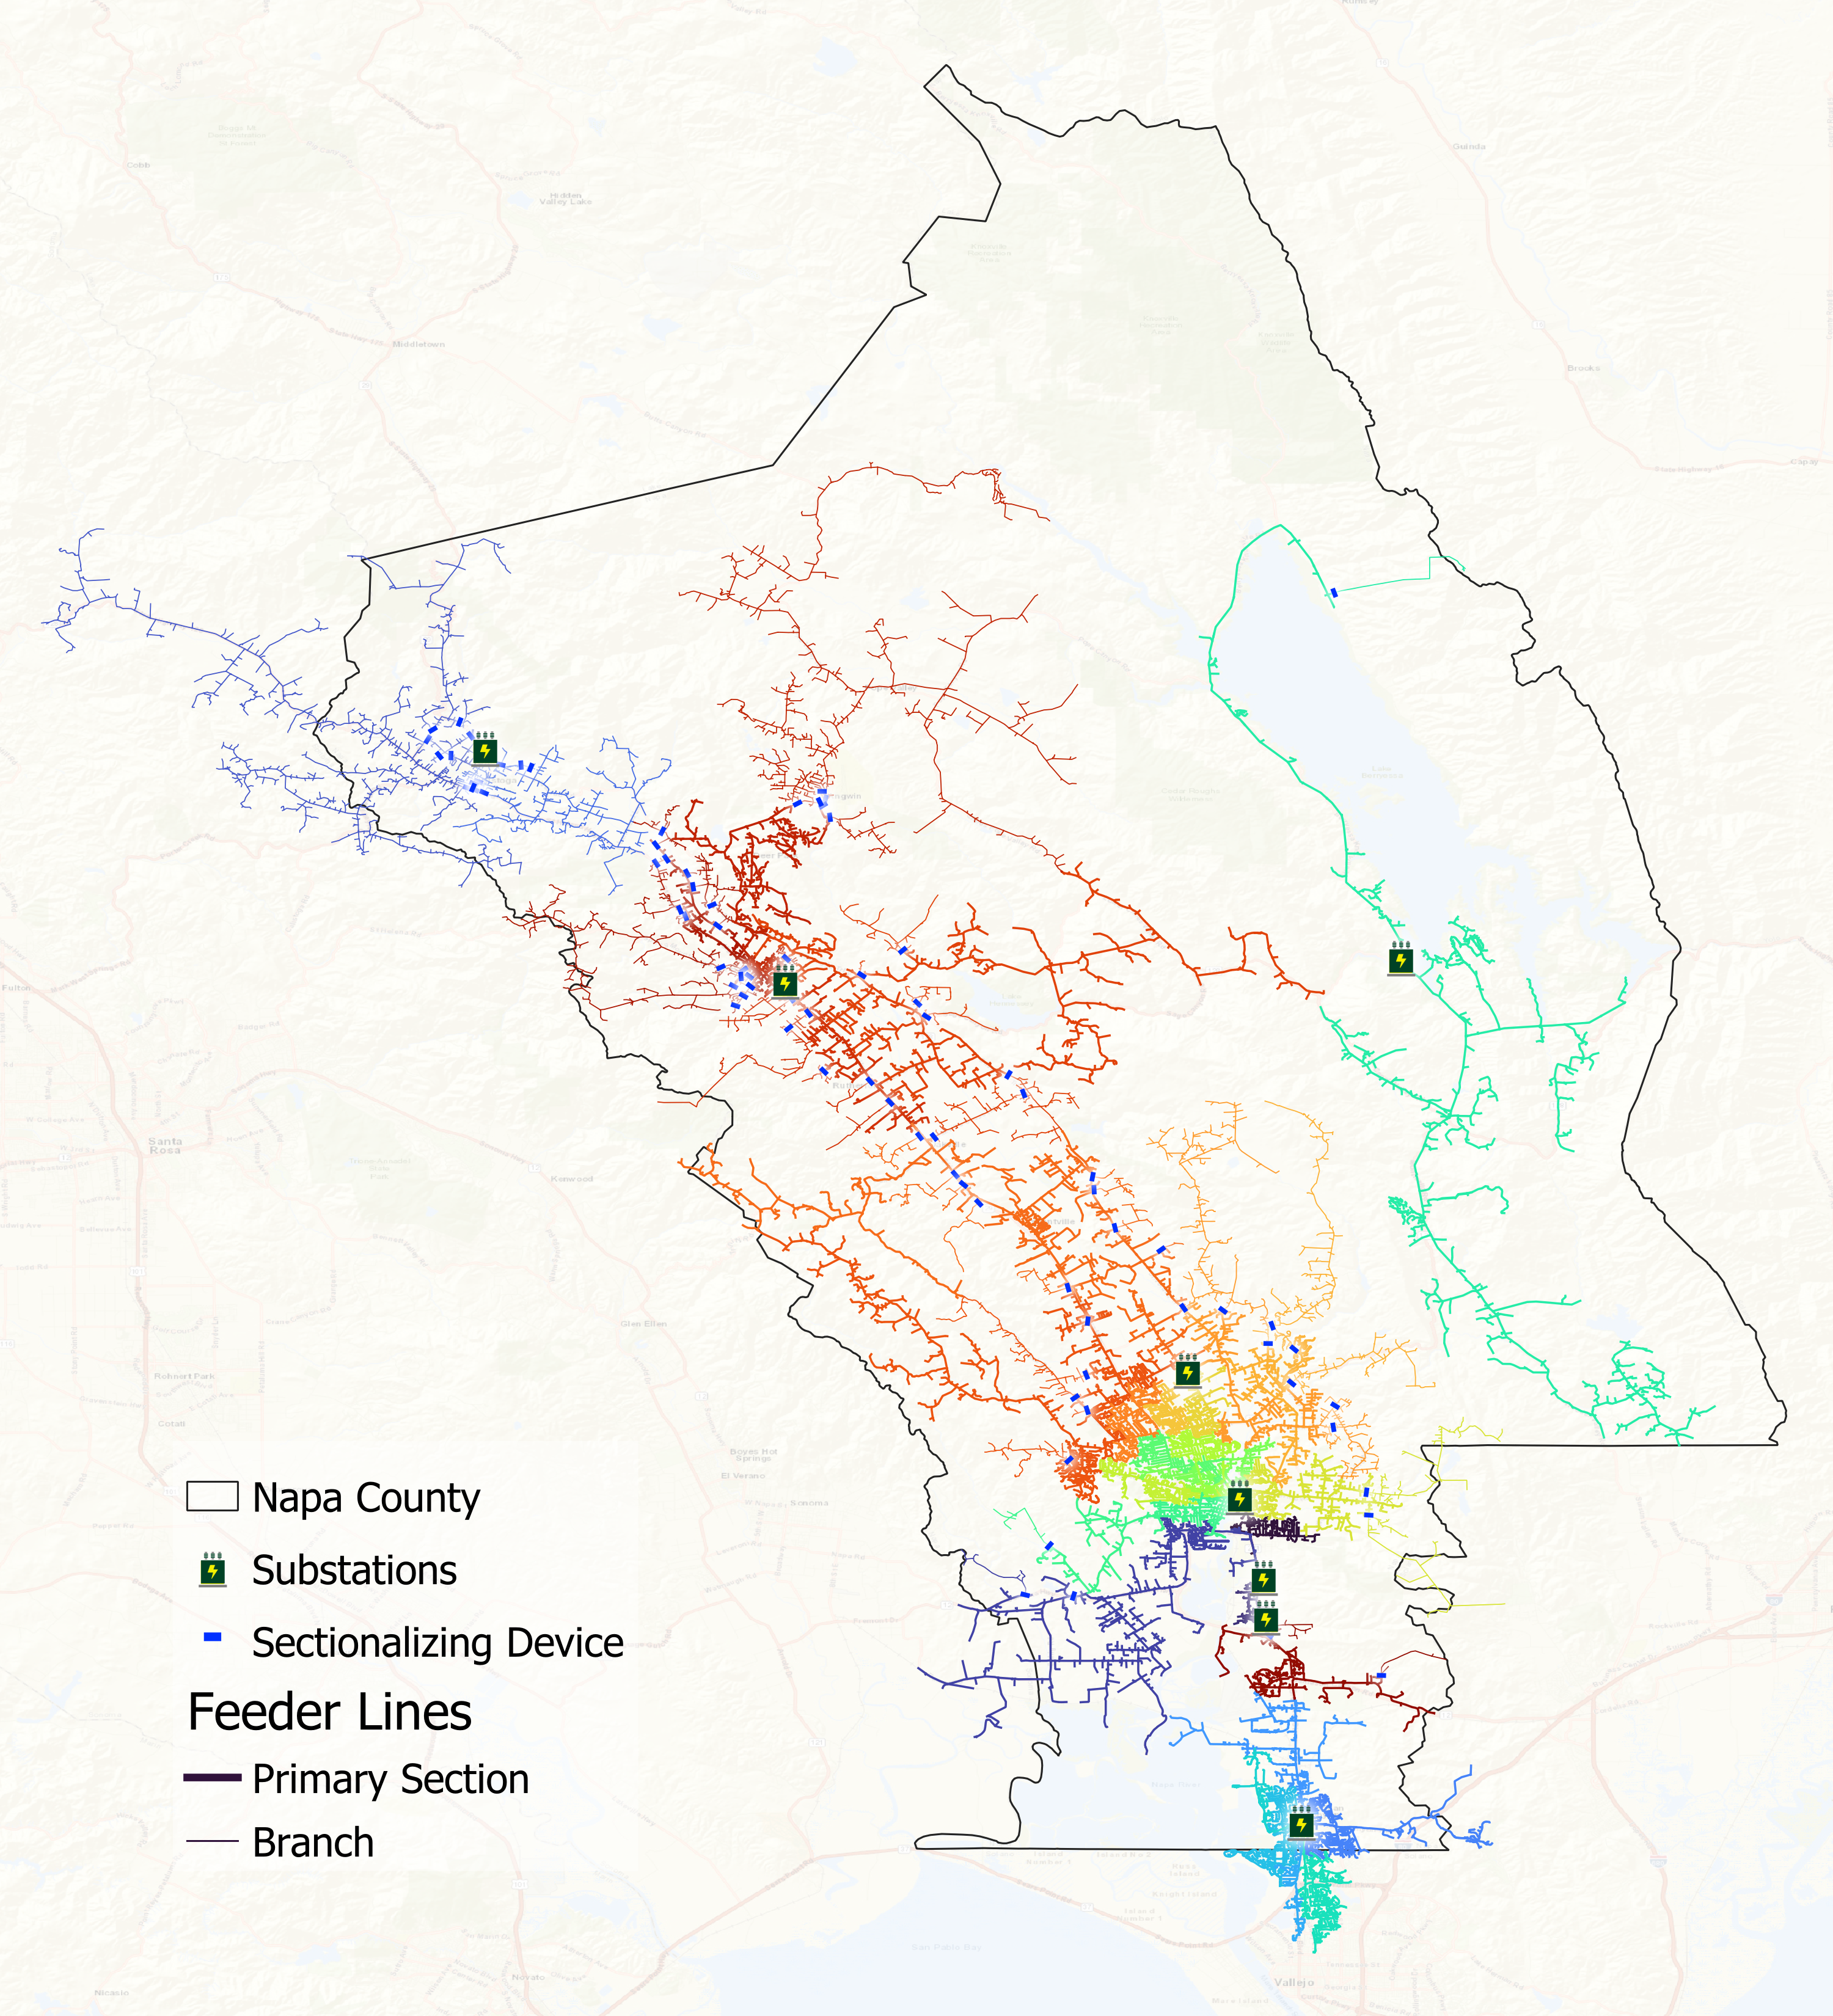
\includegraphics[height=3in]{napa_map11x10.png}
    \caption{Modeled topology of PG&E distribution system in Napa County. Feeders distinguished by line color.}
\end{figure}



\section{Napa County PSPS Simulation Results}


After building a model of the PG&E Napa county distribution system, we ran our simulation over the time period of October 15th 2021 to October 21st, 2021. In this time period an actual PSPS event was conducted by PG&E which lasted over several days and ended when a light rain greatly reduced fire risk$[7]$.  You can see in figures 5, 6, and 7 how the ignition probability increases over time in response to increases in wind, but the normalized fire potential index decreases over time in account for the rain reducing the fire potential. This drastic reduction in fire potential is what causes the number of grid sections turned on to increase, as seen in figure 7. 

This simulation was run for hyper-parameter alpha values of 0.6. The larger the hyper-parameter values represents a higher acceptance of fire risk. We examined the sensitivity of the model to the hyperparameter alpha below.


\begin{figure}[H]
    \centering
    \begin{minipage}{0.4\textwidth}
        \centering
        \includegraphics[width=.9\textwidth]{resultsmap.png}
        \caption{Lower Fire Risk timestep in Napa County Simulation}
    \end{minipage}\hfill
    \begin{minipage}{0.4\textwidth}
        \centering
        \includegraphics[width=.9\textwidth]{resultsMap2.png}
        \caption{Higher Fire Risk timestep in Napa County Simulation}
    \end{minipage}
\end{figure}


\begin{figure}[H]
    \centering
    \begin{minipage}{0.4\textwidth}
        \centering
        \includegraphics[width=1\textwidth]{IgnitionProb.png}
        \caption{Normalized Sub-feeder Ignition Probability}
    \end{minipage}\hfill
    \begin{minipage}{0.4\textwidth}
        \centering
        \includegraphics[width=1\textwidth]{FireRisk.png}
        \caption{Normalized Sub-feeder Fire Potential Index}
    \end{minipage}
\end{figure}


\begin{figure}[H]
    \centering
    \begin{minipage}{0.4\textwidth}
        \centering
        \includegraphics[width=1\textwidth]{SwitchTimeline.png}
        \caption{Number of Napa Feeder Sub-sections switch status 'on'}
    \end{minipage}
\end{figure}


\section{Outstanding Issues and Future Work}

Currently known Issues:
\begin{itemize}
\item The NOAA forecast tool gives some errors the first few time I run the script. 
\item  For some reason this always prints when you run the script but there really isn't an error I can see: ERROR [psps]: location not specified (code 1)
\item I am not using the Large Fire Probability or Fire Spread Probability options from the Geodata fire risk package. It would be low hanging fruit to include this information. I have some comments in the "importFireRiskData()" function on how you would need to filter that data.
\item Group ID definition: the system currently relies on the group ID to be defined in the JSON file and the CSV file. This was manually input into the IEEE123 JSON file and the Napa example feeder I was given. 
\item Dependencies File: The system is dependent on a "dependencies file" to define the connections between $group id$ sectionalized areas. The dependencies file is a csv which has a base "group id" field followed by a column for each other group id which the base group id is electrically connected to. This file mimic the connection constraint formula, and is directly used to construct that constraint. The source group id's (like substation connected sections) are defined with a 1 in at least one of the columns and zeros in other columns. In the future this dependencies file should be automatically generated from the JSON file by reading through the to and from fields. 
\item Normalization & aggregation-  I would like to change the aggregation and normalization process for fire risk and ignition probability. By normalizing these factors with respect to the maximum value in the 7 day forecast window as opposed to the maximum possible value, we lose out on information of the relative risk across all potential risk values outside the simulation window. One option would be to modify the $aggregateAreaData()$ function. In this function, the node level fire risk, ignition probability, and customer count data is aggregated to the group ID level via groupby and sum. The current issue with using the summing of fire risk approach is that a shorter line with extremely high fire risk  would potentially be kept on compared to a very long line with moderate fire risk. I propose using the maximum firerisk along a line or perhaps the top X\% of fire risk along a line. This should be explored and simulated with various options to more realistically model how a utility would make decisions on de-energizing a line. 
\item Optimization Formulation: the package could benefit from altering formulation to be an Goal Programming Multi-Objective optimization rather than weighted sums method. In this goal programming formulation the two objective (Minimization of fire risk and customer lost load hours) would be split between objective function and constraints. The objective function in this approach would be to minimize customer lost load hours, subject to a constraint of maximum fire risk acceptable. I believe this method is likely to be more in-line with how utilities operate where they would like to meet certain safety probability goals while constantly maximizing customer load served. 
\item OPF constraints: we don't know if the switch's being turned on or off are currently electrically feasible. To maintain electrical stability the optimal power flow constrains should be included. This would mean including information from the JSON and GIS files on line ratings etc. The current formulation could give results that could not be conducted in reality while maintaining reliability on the remainder of the distribution system. 
\item Ignition Probability Model: The current AUC score is only slightly better than a random guess. It is no surprise the logit model score so low since it is based only on wind speed. I tested one model which included tree canopy height which also scored 0.64. PG&E's distribution system ignition classification model achieves an AUC of ~0.85. This is a significant improvement, and there should be a major effort to improve this model. I have tested the MaxEnt algorithm which PG&E uses for their ignition probability model and was not able to improve the model. 
\item In the long term it would be great to be able to read directly from GIS files


\end{itemize}
After these initial improvements are made. The core of this model could be used to assess the investments in mitigating fire risks. With tuned fire risk acceptance parameters, the system could be used to test the risk reduction of investing in under-grounding power-lines or solar/storage devices.

\section{References}

$[1]$ N. Rhodes, L. Ntaimo, and L. Roald. “Balancing wildfire risk and power outages through optimized power shut-offs”. In: IEEE Transactions on Power Systems (2020).

$[2]$ https://www.cpuc.ca.gov/industries-and-topics/wildfires

$[3]$ https://dev.meteostat.net/python/#installation

$[4]$ https://www.usgs.gov/fire-danger-forecast/about-fire-danger-forecast

$[5]$ https://www.pge.com/b2b/distribution-resource-planning/integration-capacity-map.shtml

$[6]$ https://www.pge.com/en_US/residential/outages/public-safety-power-shuttoff/psps-planning-resources.page

$[7]$ https://www.pge.com/en_US/residential/outages/public-safety-power-shuttoff/psps-reports.page

$[8]$ https://data.humdata.org/dataset/united-states-high-resolution-population-density-maps-demographic-estimates

$[9]$ QGIS.org, 2022. QGIS Geographic Information System. QGIS Association. http://www.qgis.org


% \newpage
% For Poster:

% \begin{table}[h]
%     \centering
%     \begin{tabular}{c|lc}
%          Variable & Description & Unit\\
%          $x_{t,a}$ & Switch status of area $a$ at time $t$ & -- \\
%          $x_{d}$ & Switch status of area $d$ that area $a$ is & --
%          \\ & dependent on \\
%          $R_{t,a}$ & Fire Risk of area $a$ at time $t$ & -- \\
%          $C_{t,a}$ & Customers of area $a$ at time $t$ & Customer-hrs\\
%          $\alpha$ & Hyperparameter representing wildfire risk tolerance & -- \\

%          $A$ & Set of all of grid sectionalized areas & --\\
%          $T$ & Set of all timesteps & --\\
%          $D$ & Set of all grid sectionalized areas that area $a$ is & --
%          \\ & dependent on \\

%     \end{tabular}
%     \label{tab:my_label}
% \end{table}

% % ### OBJECTIVE
% \begin{equation}
%     \min_{x} {\sum_{t}^{T}\sum_{a}^{A} \;\; [x_{t,a} * R_{t,a} * (1 - \alpha) - x_{t,a} * C_{t,a} * \alpha}]
% \end{equation}


% \begin{equation}
%   s.t. \;\;\;\;\;\;\;\;\;  x_{a} \leq {\sum_{d}^{D} x_{d}}  \;\;\;\;\;  \forall \; a \in A 
% \end{equation}








\end{document}
